\documentclass[10pt]{beamer}
\usetheme{Berkeley}
\usepackage[utf8]{inputenc}
\usepackage{amsmath}
\usepackage{amsfonts}
\usepackage{amssymb}
\usepackage{graphicx}
\usepackage{ragged2e}
\setbeamercovered{transparent} 
\usecolortheme{dolphin}
\usepackage{adjustbox}
\usepackage{color}
\usepackage{listings}
\lstset{
  basicstyle=\footnotesize,
  numbers=left,
  numberstyle=\tiny\color{gray},
  stepnumber=1,
  numbersep=5pt,
  backgroundcolor=\color{white},
  showspaces=false,
  showstringspaces=false,
  showtabs=false,
  frame=single,
  rulecolor=\color{black},
  tabsize=2,
  captionpos=b,
  breaklines=true,
  breakatwhitespace=false,
  keywordstyle=\color{blue},
  commentstyle=\color{dkgreen},
  stringstyle=\color{mauve},
  escapeinside={\%*}{*)},
  otherkeywords={!=, ~, *, \&, \%/\%, \%*\%, \%\%, <-, <<-, /}
}
\definecolor{dkgreen}{rgb}{0,0.6,0}
\definecolor{gray}{rgb}{0.5,0.5,0.5}
\definecolor{mauve}{rgb}{0.58,0,0.82}
\usepackage{multirow}

\author{Russell Land}
\title[Analyzing Data on Drug Overdoses Across the US]{A Bayesian Approach to Analyze Drug Overdose Deaths Across the United States in 2018}
\institute{Georgia Southern University} 
\date{December 9, 2019} 
\subject{Introduction to Bayesian Statistics} 

\newcommand*{\Scale}[2][4]{\scalebox{#1}{$#2$}}%
\newcommand*{\Resize}[2]{\resizebox{#1}{!}{$#2$}}%
\begin{document}

\begin{frame}
\titlepage
\end{frame}

\begin{frame}
\tableofcontents
\end{frame}

\section{Abstract}
\begin{frame}
\frametitle{Abstract}
The goal of this project is to show my understanding of the course STAT 7090: Introduction to Bayesian Statistics. I found a data set online regarding drug overdose deaths, a current epidemic across the United States. The data set includes over 25,000 observations, but I slim it down considerably for this project. After organizing the data I use prior knowledge found online and the data to obtain a posterior density for the data.\\[2mm]
The second half of the project involves running a Bayesian multiple linear regression and finding statistics on the data to better understand how the response variable interacts with the covariates. The entirety of the project is done using R and OpenBUGS. The presentation is made using the \LaTeX\; typesetting language and the BibTex bibliography software tool.
\end{frame}

\section{Overview of Data}
\subsection{Data Set}
\begin{frame}
\frametitle{Source of Data}
The data used was found on {\it www.data.CDC.gov}\cite{data}. The data set includes the following variables:
	\begin{itemize}
		\item State
		\item Year
		\item Period
		\item Indicator
		\item Data.Value
		\item Percent.Complete
		\item Percent.Pending.Investigation
		\item State.Name
		\item Footnote
		\item Footnote.Symbol
		\item Predicted.Value
	\end{itemize}
\end{frame}

\begin{frame}
\frametitle{Source of Data (cont.)}
	I am interested in the variables: {\bf Data.Value}, {\bf State}, {\bf Year}, {\bf Month}, and {\bf Indicator}. The {\bf indicator} I am interested in is ``Number of Drug Overdose Deaths."\\[2mm]
	The following code will look at observations with {\bf Year} of `2018' and an {\bf indicator} of 'Number of Drug Overdose Deaths.' It will then add the number of deaths per month per state.
	\lstinputlisting[language=R,linerange={9-15}]{bayesian_project.R}
\end{frame}

\begin{frame}
\frametitle{Source of Data (cont.)}
	It takes this...\\
		\begin{center}
		\begin{tabular}{|c|c|c|}
			\hline
			State & Month & Data.Value\\
			\hline
			AK & January & 46\\
			\hline
			AK & February & 30\\
			\hline
			AK & March & 26\\
			\hline
			\vdots & \vdots\ & \vdots\\
			\hline
			AK & December & 25\\
			\hline
		\end{tabular}
		\end{center}
	and turns it into...
		\begin{center}
		\begin{tabular}{|c|c|}
			\hline
			State & Data.Value\\
			\hline
			AK & 412\\
			\hline
		\end{tabular}
		\end{center}
\end{frame}

\subsection{Variables}
\begin{frame}
	The next step is to size this data to something easier to work with and something applicable. Next, I add the population of each state\cite{state}, the region of every state\cite{region}, the annual income per capita per state\cite{income}, and the health care expenditures per capita by state residence\cite{health}.\\[4mm]
	So why did I choose these variables to add to the data?
\end{frame}

\begin{frame}
	\frametitle{Population of Each State}
I start with the number of deaths for each state ($n_i$) and the population of each state ($N_i$). Dividing the two will give the ratio ($r_i$) of deaths per state: $$r_i=\frac{n_i}{N_i}.$$ After this I multiply the ratio by 100 to give the percentage, which makes the data easier to read. With this following transformation, the data now looks like...
	\begin{center}
	\begin{adjustbox}{width=\columnwidth,center}
	\begin{tabular}{|c|c|c|c|c|}
		\hline
		Number & State & Number of Deaths $(n_i)$ & Population $(N_i)$ & Ratio $(\%)$\\
		\hline
		1 & AK & 412 & 737,438 & 0.055869104\\
		\hline
		2 & AL & 2632 & 4,887,871 & 0.053847575\\
		\hline
		3 & AR & 1718 & 3,013,825 & 0.057003973\\
		\hline
		\vdots & \vdots & \vdots & \vdots & \vdots\\
		\hline
		51 & WY & 103 & 577,737 & 0.017828181\\
		\hline
	\end{tabular}
	\end{adjustbox}
	\end{center}
\end{frame}

\begin{frame}
\frametitle{Regions}
	I classify each state into a region. Just a brief glance at the data I notice a higher trend of deaths in the eastern United States; they may have a linear relationship. Here is how I classified each state. Note that I classify Alaska in region 1 and Hawaii in region 2.
	\begin{center}
	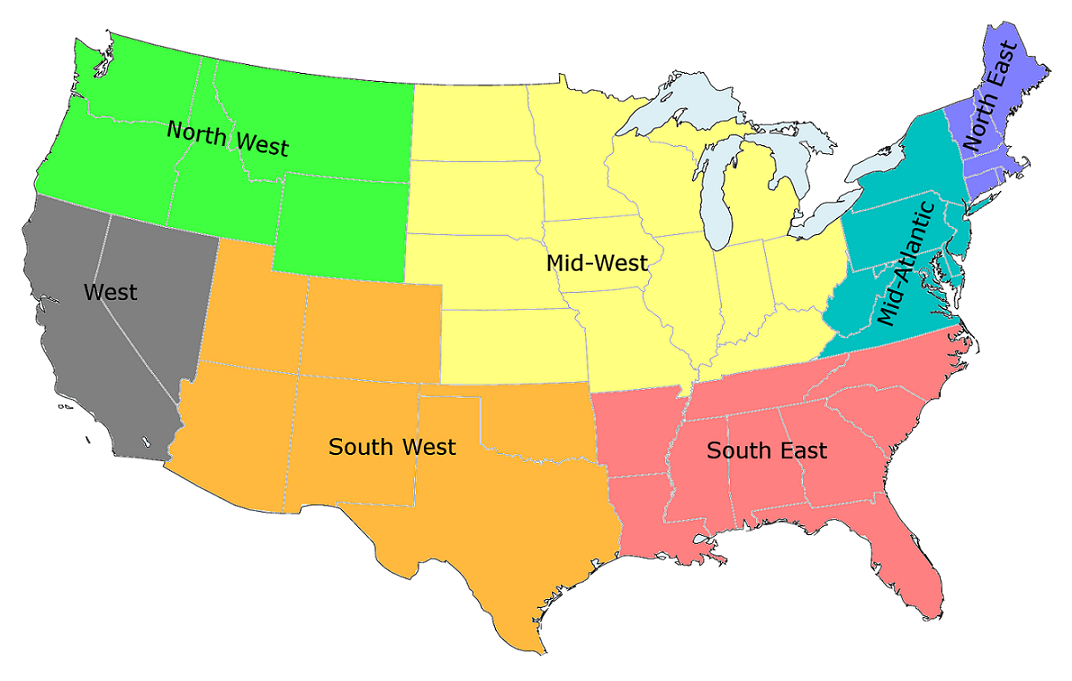
\includegraphics[scale=0.25]{regions.png}\\
	Figure 1: Regions of the USA\cite{region}
	\end{center}
\end{frame}

\begin{frame}
\frametitle{Income}
	I include the variable `household median incomes per capita per state'\cite{income}. My reasoning behind this, is the idea that the level of an individuals income could be related to their potential to abuse illegal or prescription drugs. Here are a few of the observations:
		\begin{center}
		\begin{tabular}{|c|c|c}
			\hline
			State & Income (\$)\\
			\hline
			AK & 73,181\\
			\hline
			AL & 48,123\\
			\hline
			AR & 45,869\\
			\hline
			\vdots & \vdots\\
			\hline
			WY & 60,434\\
			\hline
		\end{tabular}
		\end{center}
\end{frame}

\begin{frame}
\frametitle{Health Care}
	The last variable I add is health care expenditures per capita of each state. The more a state spends on health care should be related to how many prescription drugs are purchased, right? We will test this.\\[2mm]
	With all this being said, here is a summary of the data I will be working with.
		\begin{center}
		\begin{adjustbox}{width=\columnwidth,center}
		\begin{tabular}{|c|c|c|c|c|c|c|}
		\hline
		Number & State & Deaths & Percent.Pop & Region & Income (\$) & Health.Care (\$)\\
		\hline
		1 & AK & 412 & 0.055869104 & 1 & 73,181 & 11,064\\
		\hline
		2 & AL & 2,632 & 0.053847575 & 5 & 48,123 & 7,281\\
		\hline
		3 & AR & 1,718 & 0.057003973 & 5 & 45,869 & 7,408\\
		\hline
		\vdots & \vdots & \vdots & \vdots & \vdots & \vdots & \vdots\\
		\hline
		51 & WY & 103 & 0.017828181 & 1 & 60,434 & 8,320\\
		\hline
		\end{tabular}
		\end{adjustbox}
		\end{center}
\end{frame}

\section{Brief Frequentist Approach}
\begin{frame}
\frametitle{Frequentist Approach}
	I know this is a Bayesian project, but I will run a frequentist analysis to get a feel for the data. Then we can compare the frequentist approach and Bayesian approach at the end. I ran the following code and got the output below.
		\lstinputlisting[language=R,linerange={49-50}]{bayesian_project.R}
		\texttt{
		\begin{adjustbox}{width=\columnwidth,center}
		\begin{tabular}{l}
			Call:\\
			lm(formula = data2[,3] ~ data2[,4] + data2[,5] + data2[,6])\\
		\end{tabular}
		\end{adjustbox}
		\begin{adjustbox}{width=\columnwidth,center}
		\begin{tabular}{rrrrr}
			\hline
			Coefficients: & & & &\\
			& Estimate & Std. Error & t value & Pr($>|t|$)\\
			(Intercept) & -1.931e-02 & 3.178e-02 & -0.608 & 0.5463\\
			data2[,4] & 6.682-e03 & 2.633e-03 & 2.538 & 0.0145\\
			data2[,5] & -2074e-07 & 4.545e-07 & -0.456 & 0.6503\\
			data2[,6] & 7.711e-06 & 4.141e-06 & 1.862 & 0.0688\\
			\hline
		\end{tabular}
		\end{adjustbox}
		\begin{adjustbox}{width=\columnwidth,center}
		\begin{tabular}{llll}
			Multiple R-squared: & 0.2841, & Adjusted R-squared: & 0.2384
		\end{tabular}
		\end{adjustbox}
		}
\end{frame}

\begin{frame}
\frametitle{Frequentist Approach (cont.)}
	We will now only include the first covariate (region), because it is the only significant one.
	\lstinputlisting[language=R,linerange={51-52}]{bayesian_project.R}
		\texttt{
		\begin{adjustbox}{width=\columnwidth,center}
		\begin{tabular}{llllll}
			Call:&     &     &    &    &    \\
			lm(formula = data2[,3] ~ data2[,4])&    &    &    &    &    \\
		\end{tabular}
		\end{adjustbox}
		\begin{adjustbox}{width=\columnwidth,center}
		\begin{tabular}{rrrrr}
			\hline
			Coefficients: & & & &\\
			& Estimate & Std. Error & t value & Pr($>|t|$)\\
			(Intercept) & 0.022503 & 0.010907 & 2.063 & 0.044416\\
			data2[,4] & 0.009023 & 0.002362 & 3.819 & 0.000377\\
			\hline
		\end{tabular}
		\end{adjustbox}
		\begin{adjustbox}{width=\columnwidth,center}
		\begin{tabular}{llll}
			Multiple R-squared: & 0.2294, & Adjusted R-squared: & 0.2137
		\end{tabular}
		\end{adjustbox}
		}
\end{frame}

\begin{frame}
\frametitle{Frequentist Approach (cont.)}
	Here are scatterplots for (deaths vs. ratios), (ratios vs. region), (ratio vs. income), and (ratio vs. health care).
	\begin{center}
	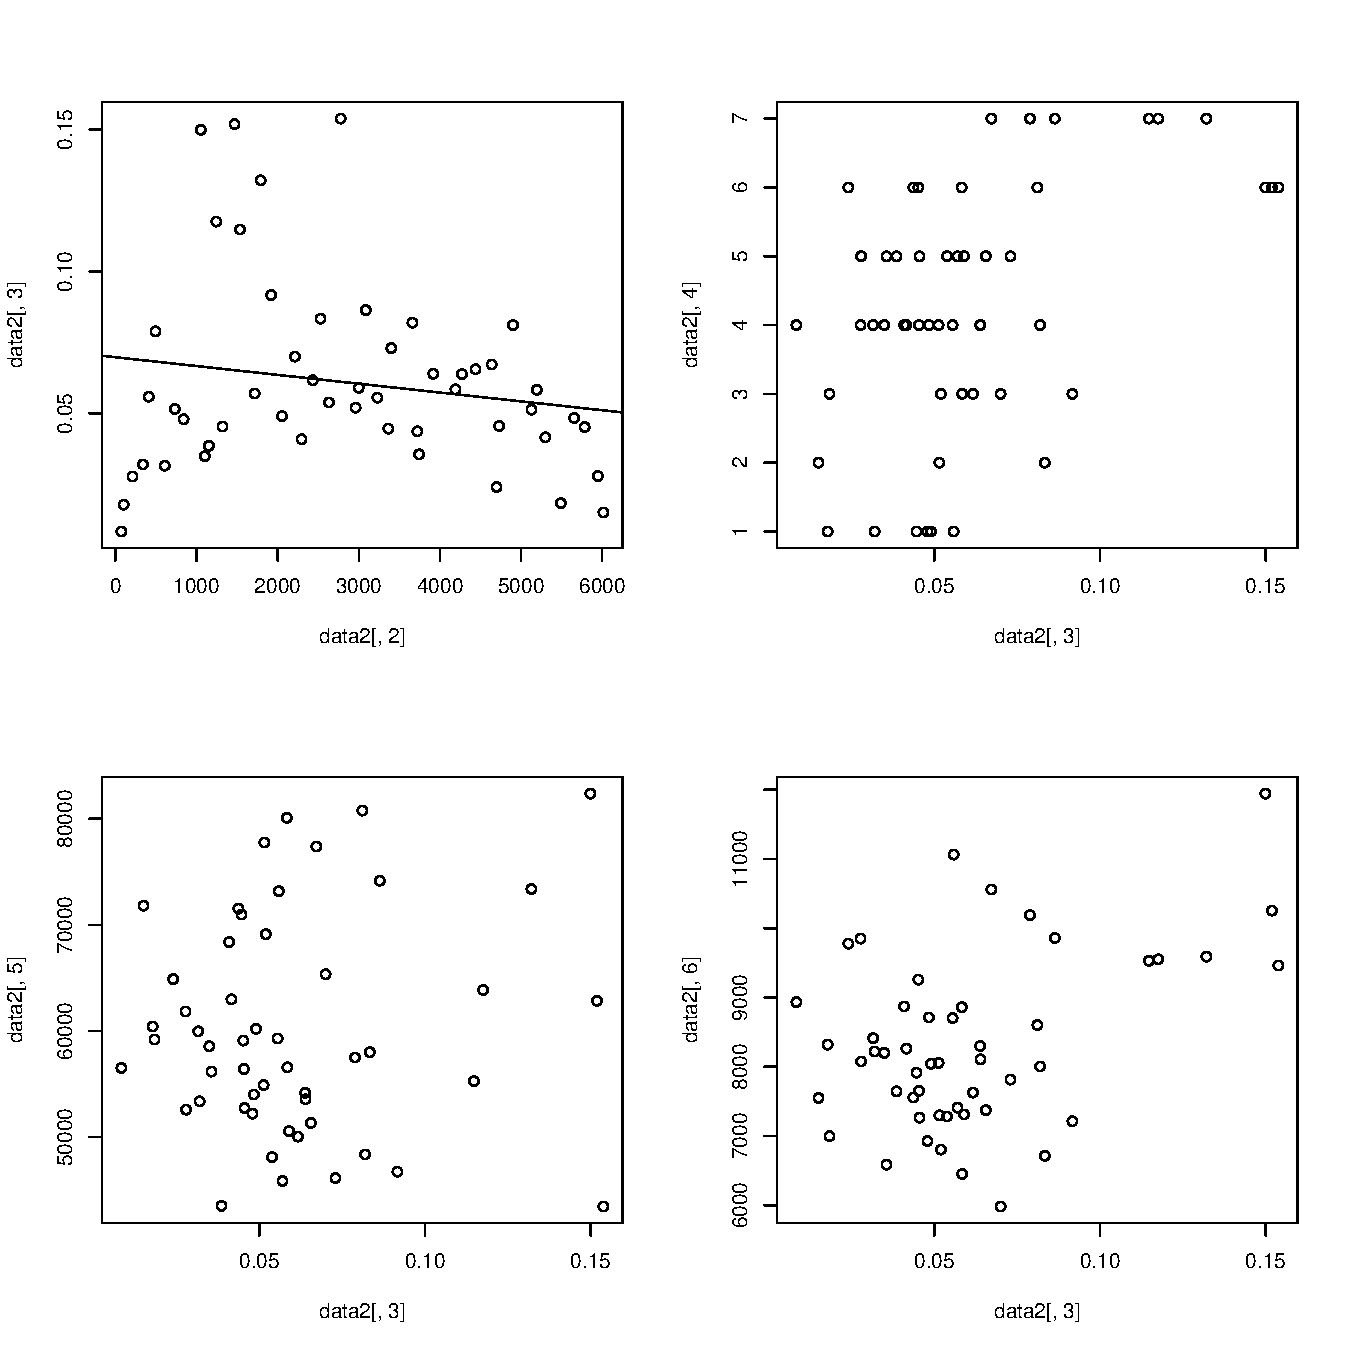
\includegraphics[scale=0.25]{linreg1.pdf} 
	\end{center}
\end{frame}

\section{Bayesian Approach}
\subsection{Posterior Density}
\begin{frame}
\frametitle{Posterior Density}
Before we begin a posterior density calculation we need to make some assumptions about the data.
	\begin{itemize}
		\item We will assume the data is distributed normally with mean $\theta$ and known standard deviation $\sigma$.
		\item We are going to assume prior knowledge about this data. In an article about the predictions of 2018 data, there was an estimate that every 58 out of 100,000 people in the United States will die from a drug overdose in 2018\cite{article}. We will choose a normal prior with mean 0.058 and standard deviation of 0.5. These were picked by analyzing data from 2017.
		\item Unrelated to our study, about 7 out of 10 of these overdose deaths come from opioids such as fentanyl, heroin, and prescription opioids\cite{article}.
	\end{itemize}
\end{frame}

\begin{frame}
\frametitle{Posterior Density Derivation}
	This distribution is one that we derived in class. I will include the derivation below. We know that a posterior density can be obtain with the following: $$\pi(\theta|y)=\frac{f(y|\theta)\cdot\pi(\theta)}{m(y)}$$ where $$m(y)=\int_{\theta}f(y|\theta)\cdot\pi(\theta)d\theta$$ Let's also mention that both the likelihood function and prior belong to the exponential family, and thus are conjugate distributions.
\end{frame}

\begin{frame}
\frametitle{Posterior Density Derivation (cont.)}
	The likelihood function is $$f(y|\theta)=\frac{1}{\sigma\sqrt{2\pi}}\exp\left\{-\frac{1}{2\sigma^2}\left(y-\theta\right)^2\right\}$$ and the prior in terms of $\theta$ is $$\pi(\theta)=\frac{1}{\tau_0\sqrt{2\pi}}\exp\left\{-\frac{1}{2\tau_0^2}\left(\theta-\mu_0\right)^2\right\}$$ where $\mu_0$ are $\tau_0$ are hyper-parameters.
\end{frame}

\begin{frame}
\frametitle{Posterior Density Derivation (cont.)}
	\begin{align*}
		\pi(\theta|y)&=\frac{\overbrace{f(y|\theta)\cdot\pi(\theta)}^{n}}{\int_{\theta}f(y|\theta)\cdot\pi(\theta)d\theta}\\
		n&=\frac{1}{\sigma\sqrt{2\pi}}\exp\left\{-\frac{1}{2\sigma^2}\left(y-\theta\right)^2\right\}\cdot\frac{1}{\tau_0\sqrt{2\pi}}\exp\left\{-\frac{1}{2\tau_0^2}\left(\theta-\mu_0\right)^2\right\}\\
		&=\frac{1}{2\pi\sigma\tau_0}\exp\left\{-\frac{1}{2\sigma^2}\left(y-\theta\right)^2-\frac{1}{2\tau_0^2}\left(\theta-\mu_0\right)^2\right\}\\
		&=\frac{1}{2\pi\sigma\tau_0}\exp\left\{-\frac{1}{2\sigma^2}\left(y^2-2y\theta+\theta^2\right)-\frac{1}{2\tau_0^2}\left(\theta^2-2\theta\mu_0+\mu_0^2\right)\right\}\\
		&=\underbrace{\frac{1}{2\pi\sigma\tau_0}}_{C}\exp\bigg\{\frac{2\theta y\tau_0^2+2\theta\mu_0\sigma^2-\theta^2\left(\tau_0^2+\sigma^2\right)}{2\sigma^2\tau_0^2}-\underbrace{\frac{y^2\tau_0^2+\mu_0^2\sigma^2}{2\sigma^2\tau_0^2}}_{C_1}\bigg\}
	\end{align*}
\end{frame}

\begin{frame}
\frametitle{Posterior Density Derivation (cont.)}
	\begin{align}
		&{\tiny =C\cdot\exp\left\{\frac{-\left(\tau_0^2+\sigma^2\right)\bigg(\theta^2-2\theta\overbrace{\left(y\tau_0^2+\mu_0\sigma^2\right)\left(\tau_0^2+\sigma^2\right)^{-1}}^{B}+B^2-B^2\bigg)}{2\sigma^2\tau_0^2}-C_1\right\}}\nonumber\\
		&=C\cdot\exp\left\{\frac{\left(\tau_0^2+\sigma^2\right)B^2}{2\sigma^2\tau_0^2}-\frac{\left(\tau_0+\sigma^2\right)\left(\theta-B\right)^2}{2\sigma^2\tau_0^2}-C_1\right\}\nonumber\\
		&=C_2\cdot\exp\left\{-\frac{\left(\tau_0+\sigma^2\right)\left(\theta-B\right)^2}{2\sigma^2\tau_0^2}\right\}
	\end{align}
	where $$C_2=\frac{1}{2\pi\sigma\tau_0}\exp\left\{\frac{\left(\tau_0^2+\sigma^2\right)B^2-y^2\tau_0^2-\mu_0^2\sigma^2}{2\sigma^2\tau_0^2}\right\}$$
\end{frame}

\begin{frame}
\frametitle{Posterior Density Derivation (cont.)}
Re-expressing equation (1) slightly will give: $$\pi(\theta|y)=C_2\cdot\exp\left\{-\frac{\left(\frac{1}{\tau_0^2}+\frac{1}{\sigma^2}\right)\left(\theta-B\right)^2}{2}\right\}$$ which looks like the kernel of a normal distribution will mean $B$ and precision $\left(\frac{1}{\tau_0^2}+\frac{1}{\sigma^2}\right)$, leaving us with the constant $C_2$. Now, let's consider the denominator $m(y)$:
	\begin{align}
		m(y)&=\int_{\theta}f(y|\theta)\cdot\pi(\theta)d\theta\nonumber\\
		&=\int_{\theta}C_2\cdot\exp\left\{-\frac{\left(\frac{1}{\tau_0^2}+\frac{1}{\sigma^2}\right)\left(\theta-B\right)^2}{2}\right\}d\theta\\
		&=C_2\cdot\sqrt{2\pi\left(\frac{1}{\tau_0^2}+\frac{1}{\sigma^2}\right)^{-1}}\nonumber
	\end{align}
\end{frame}

\begin{frame}
\frametitle{Posterior Density Derivation (cont.)}
	we arrive at equation (2) using the same exact steps as before. From here we have obtained the posterior distribution. We can conclude $$\pi(\theta|y)\sim N\left(\frac{\frac{y}{\sigma^2}+\frac{\mu_0}{\tau_0^2}}{\frac{1}{\sigma^2}+\frac{1}{\tau_0^2}}\;,\;\left(\frac{1}{\sigma^2}+\frac{1}{\tau_0^2}\right)^{-1}\right)$$
\end{frame}

\begin{frame}
\frametitle{Visualization}
	With the posterior we just found, we can now make plots using the data. Below is a plot containing the likelihood, prior, and posterior. I also include a density estimation using a built-in R function. A vertical line is placed at the max of every curve to help see the differences.\vspace*{-5mm}
		\begin{center}
		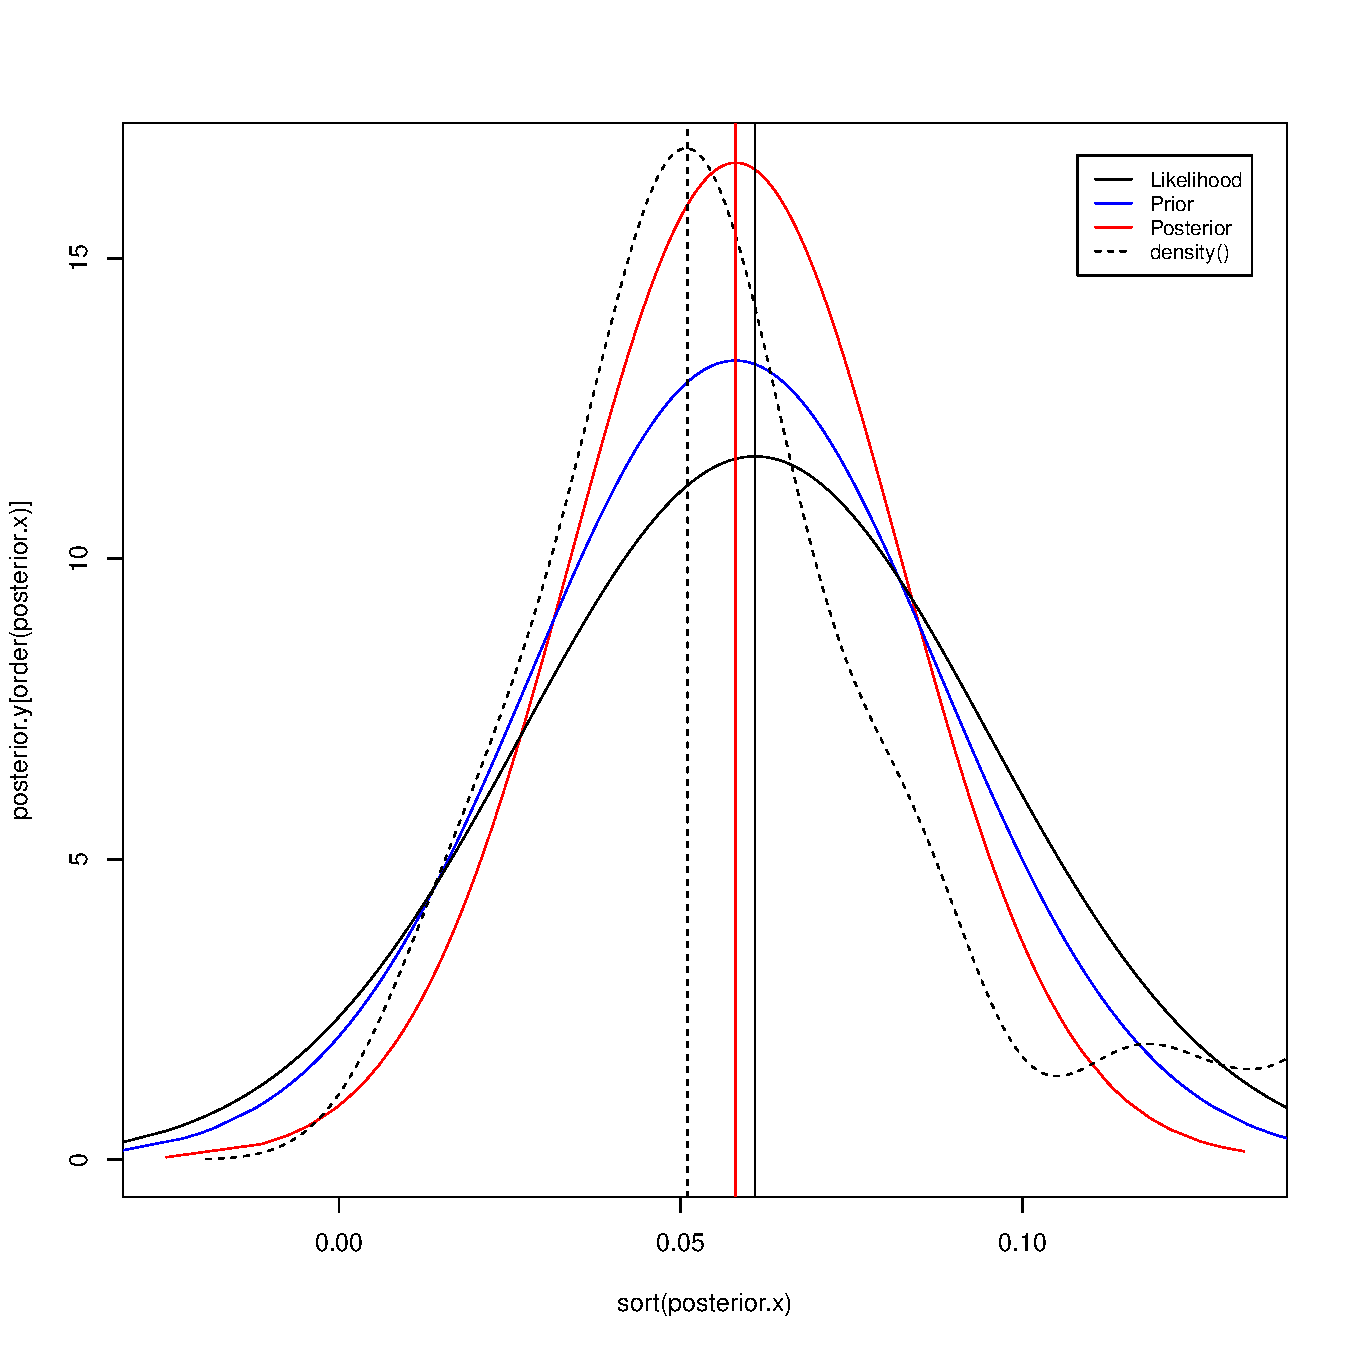
\includegraphics[scale=0.25]{posteriors.pdf} 
		\end{center}
\end{frame}

\subsubsection{MCMC Sampling}
\begin{frame}
\frametitle{MCMC Sampling}
	We were able to find the posterior density, and OpenBUGS can handle our model, but I will run an algorithm in R anyway. I will use the Metropolis-Hastings algorithm. This algorithm can be broken down into the following steps:
		\begin{enumerate}
			\item Pick an arbitrary density, say $q(\theta|\phi)$, to suggest transition probabilities.
			\item Next, we will initialize a $\theta$ value, say $\theta_0$.
			\item At time $i$, we will generate $\theta^{*}$ from the density $q\left(\theta^{*}|\theta_{i-1}\right)$.
			\item Next, the acceptance probability can be calculated by $$\alpha=\min\left(1,\frac{P\left(\theta^{*}\right)\cdot q\left(\theta_{i-1}|\theta^{*}\right)}{P\left(\theta_{i-1}\right)\cdot q\left(\theta^{*}|\theta_{i-1}\right)}\right)\qquad\text{where}\;P(\cdot)=\pi(\theta|y)$$
			\item Generate $U$ from a uniform distribution $(0,1)$.
			\item If $U\leq\alpha$, then let $\theta_{i-1}=\theta^{*}$. Otherwise let $\theta_{i+1}=\theta_i$.
			\item Repeat this process for $N$ iterations.
		\end{enumerate}
\end{frame}

\begin{frame}
\frametitle{Metropolis-Hastings Algorithm}
	\lstinputlisting[language=R,linerange={91-100}]{bayesian_project.R}
\end{frame}

\begin{frame}
\frametitle{Metropolis-Hastings Algorithm (cont.)}
	\lstinputlisting[language=R,linerange={102-120}]{bayesian_project.R}
\end{frame}

\begin{frame}
\frametitle{Metropolis-Hastings Algorithm (cont.)}
	Burn-in step not included.
	\lstinputlisting[language=R,linerange={126-141}]{bayesian_project.R}
\end{frame}

\begin{frame}
\frametitle{Metropolis-Hastings Algorithm Output}
	\begin{center}
	Density Plot\\
	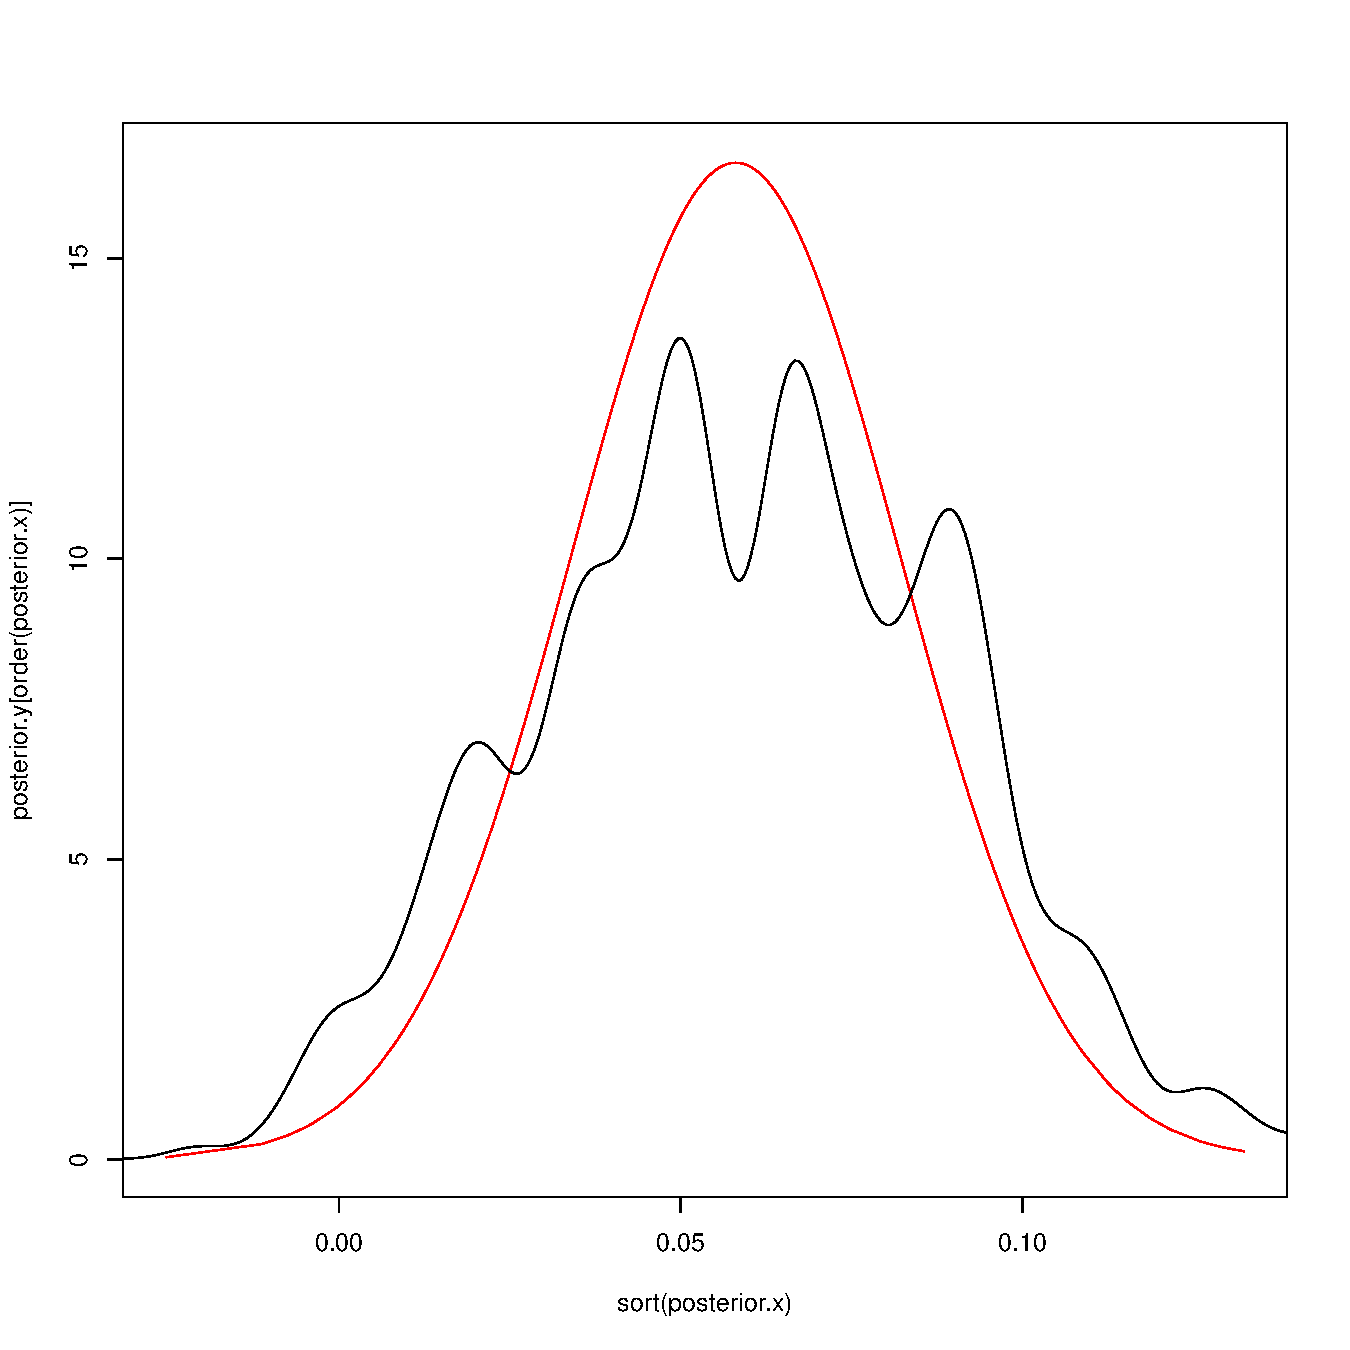
\includegraphics[scale=0.3]{metropolis.pdf}
	\end{center}
\end{frame}

\begin{frame}
\frametitle{Metropolis-Hastings Algorithm Output}
	\begin{center}
	History Plots\\
	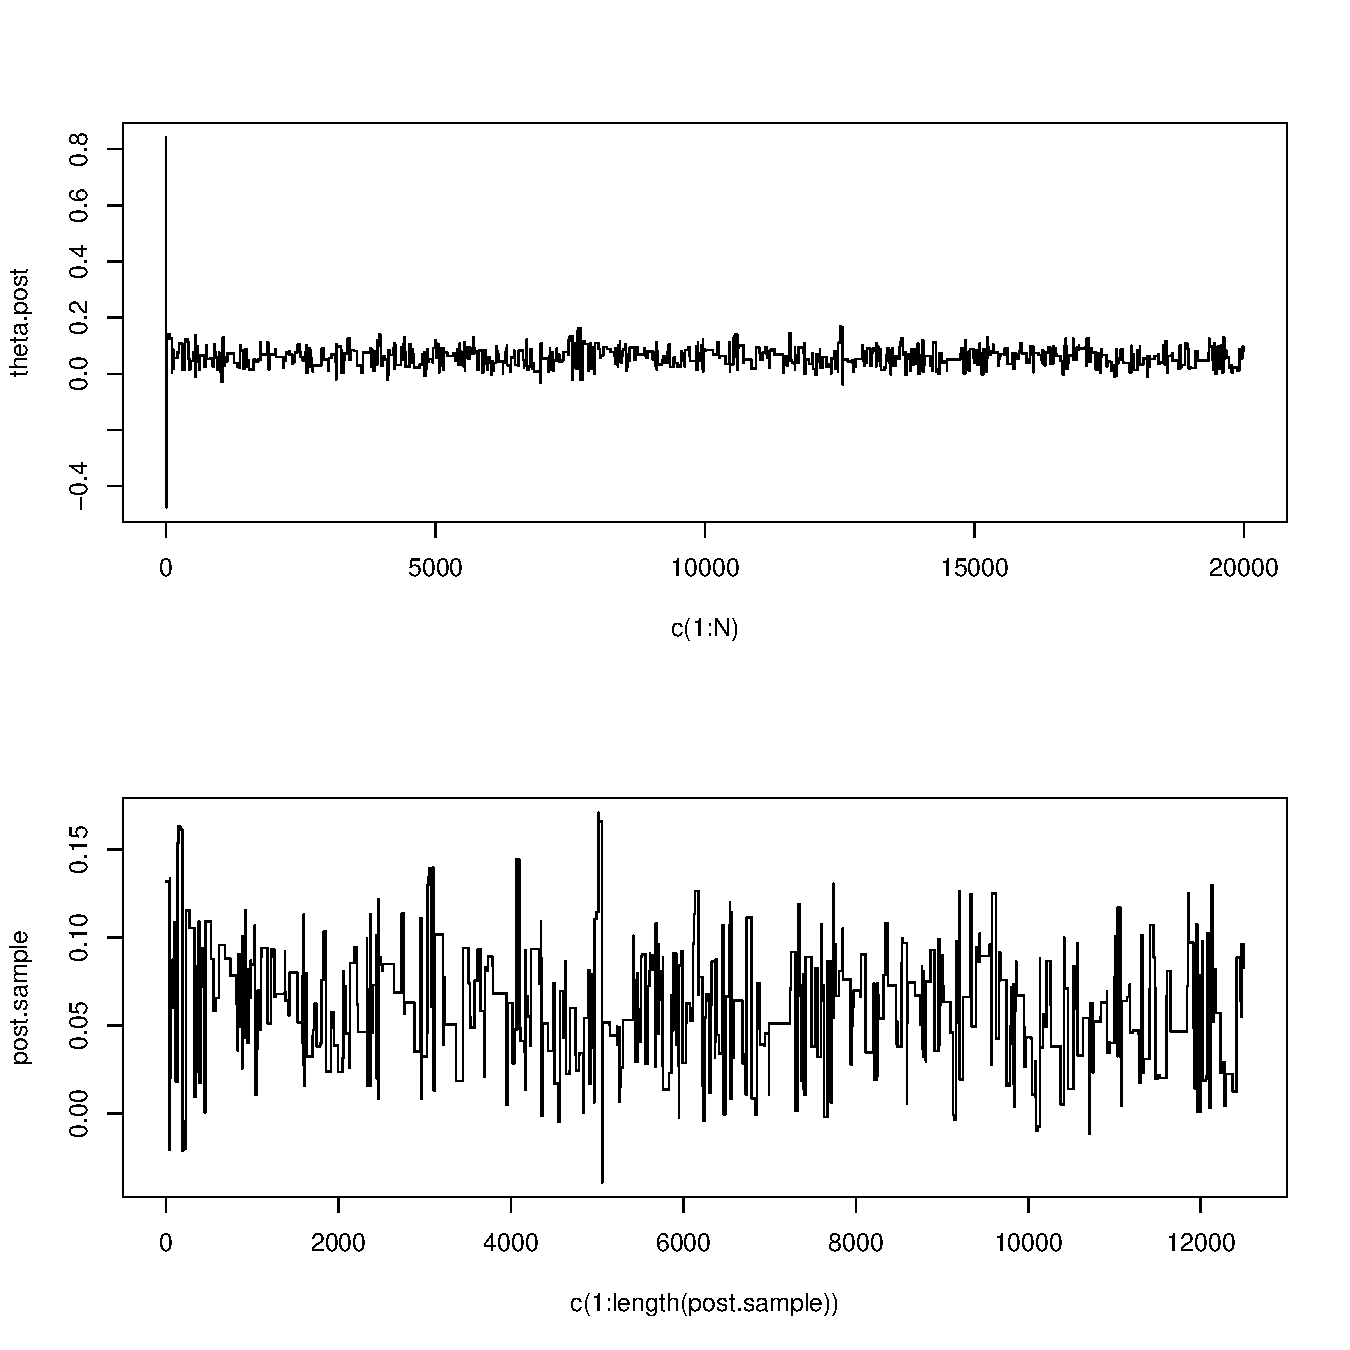
\includegraphics[scale=0.3]{history.pdf} 
	\end{center}
\end{frame}

\subsubsection{OpenBUGS}
\begin{frame}
\frametitle{OpenBUGS Posterior Density Estimation}
	We can use OpenBUGS to estimate a posterior density. Here is the model I constructed:
		\lstinputlisting[language=R,linerange={155-163}]{bayesian_project.R}
\end{frame}

\begin{frame}
\frametitle{OpenBUGS Posterior Density Estimation Output}
	\begin{center}
	Posterior Density vs. OpenBUGS Estimation\\
	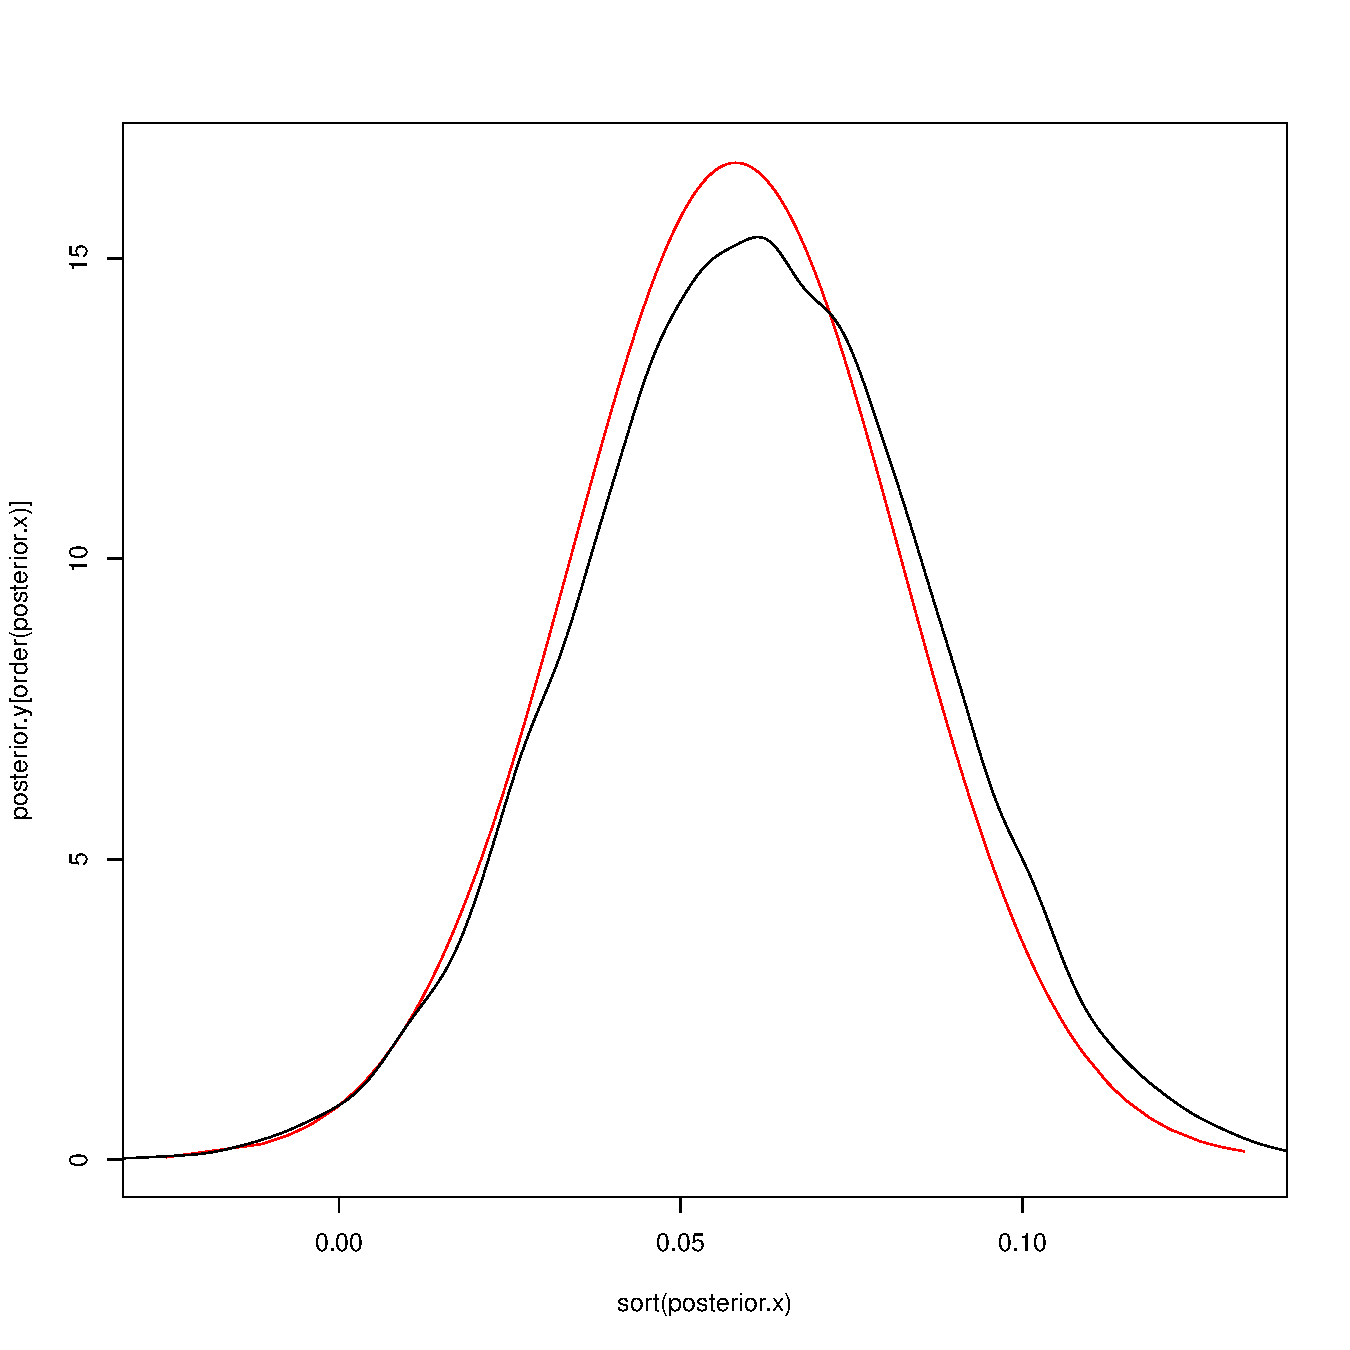
\includegraphics[scale=0.3]{openbugs.pdf} 
	\end{center}
\end{frame}

\begin{frame}
\frametitle{Some Statistics on OpenBUGS Density Estimation}
	With the density that OpenBUGS created, we can see it is a pretty close match to our calculated posterior. Let's now show the 95\% credible interval and the highest posterior density (HPD) and interpret them. The 95\% credible interval can be constructed with the following code:
	\lstinputlisting[language=R,linerange={181-181,183-187}]{bayesian_project.R}
So, 95\% of a future annual drug overdose ratio will be between the interval \texttt{(0.01081,0.11110)}. This is a fairly large interval.
\end{frame}

\begin{frame}
\frametitle{Some Statistics on OpenBUGS Density Estimation}
	The HPD interval can be constructed with a built-in function, but here is code that I made:
		\lstinputlisting[language=R,linerange={196-212}]{bayesian_project.R}
\end{frame}

\begin{frame}
\frametitle{Some Statistics on OpenBUGS Density Estimation}
	\lstinputlisting[language=R,linerange={214-233}]{bayesian_project.R}
\end{frame}

\begin{frame}
\frametitle{Some Statistics on OpenBUGS Density Estimation}
	\lstinputlisting[language=R,linerange={234-255}]{bayesian_project.R}
\end{frame}

\begin{frame}
\frametitle{Some Statistics on OpenBUGS Density Estimation}
	The highest density interval is the narrowest interval that includes the highest probability possible at 95\%. Below is a visual of this.
	\begin{center}
	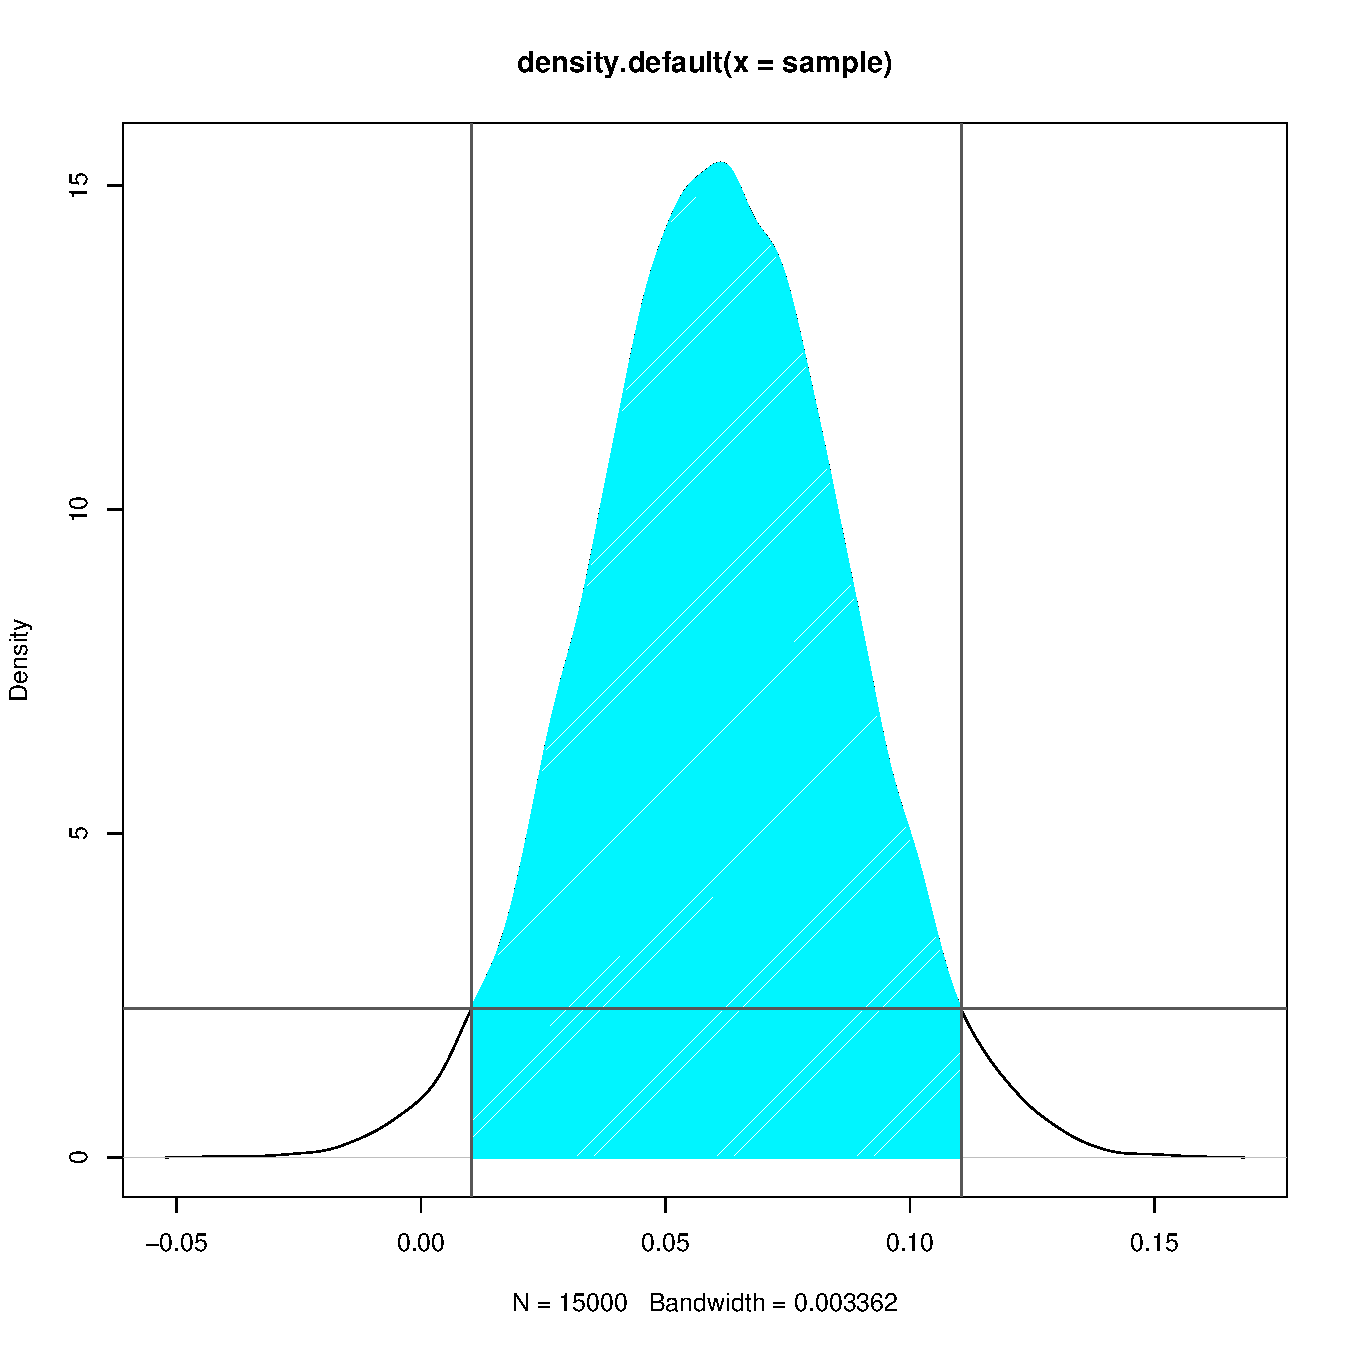
\includegraphics[scale=0.3]{hdi.pdf} 
	\end{center}
\end{frame}

\subsection{Multiple Linear Regression}
\begin{frame}
\frametitle{Bayesian Linear Regression}
	Next in our analysis I will run a Bayesian multiple linear regression on the response variable `number of deaths' with covariates `region', 'income per capita per state', and 'health care expenditures per capita per state'.\\[2mm]
	The goal of this multiple linear regression is to answer the following questions:
		\begin{enumerate}
			\item How does the response variable vary as as function of the covariates?
			\item Which $X_j$'s have an effect?
			\item Can we predict $Y$ as a function of $X$?
		\end{enumerate}
	These are questions I will answer. Because we are taking a Bayesian approach we will test three different priors, two shrinking priors and one flat prior. The shrinking priors will tell us the significant covariates. I will start with Zellner's g-prior.
\end{frame}

\begin{frame}
\frametitle{Zellner's G-Prior}
	We first need to initialize our response variable and covariates. This prior involves a variance-covariance matrix, so we need to calculate that as well. Here is the code for that:
		\lstinputlisting[language=R,linerange={266-274}]{bayesian_project.R}
	The next slide will contain the model.
\end{frame}

\begin{frame}
\frametitle{Zellner's G-Prior (cont.)}
	\lstinputlisting[language=R,linerange={276-293}]{bayesian_project.R}
\end{frame}

\begin{frame}
\frametitle{Zellner's G-Prior (cont.)}
	\lstinputlisting[language=R,linerange={295-305}]{bayesian_project.R}
	Here is the regression equation for this model: $$\hat{Y}=-0.019+0.006X_1-0.000X_2+0.000X_3$$ The last two coefficients are very small. This is a trend that continues for all of the models I test.
\end{frame}

\begin{frame}
\frametitle{Other Prior Choices}
	I ran the following priors using all three covariates and then again with the same priors, but with only the first covariate, `regions'.
		\begin{itemize}
			\item Zellner's G-Prior
			\item Double Exponential Prior
			\item Flat Prior
		\end{itemize}
	I am not going include all of the models, but I will list the regression equation for each.
\end{frame}

\begin{frame}
\frametitle{Regression Equations}
	\begin{itemize}
		\item Zellner's G-Prior (three covariates) $$\hat{Y}=-0.019+0.006X_1-0.000X_2+0.000X_3$$
		\item Double Exponential Prior (three covariates) $$\hat{Y}=298.126+49.401X_1+0.016X_2-0.179X_3$$
		\item Flat Prior (three covariates) $$\hat{Y}=-0.012+0.007X_1-0.000X_2+0.000X_3$$
		\item Zellner's G-Prior (one covariate) $$\hat{Y}=0.022+0.008X_1$$
		\item Double Exponential (one covariate) $$\hat{Y}=0.228+0.008X_1$$
		\item Flat Prior (one covariate) $$\hat{Y}=0.023+0.008X_1$$
	\end{itemize}
\end{frame}

\subsubsection{Model Comparison}
\begin{frame}
\frametitle{Model Comparison}
	After running multiple models, how can we decide which one is superior?\\[2mm]
	We have a few ways for model comparison. We can use LPML, or log-psuedo-marginal-likelihood. This is a type of `leave-one-out' cross-validation. This process esentially works by running the model and leaving out an observation each time. After running the model $n$ times, calculate the conditional predictive ordinate, usually abbreviated by cpo. We denote it as $$\text{cpo}_j=P\left(y_1|y_{(-1)}\right)=\int_{\theta}f\left(y_1|\theta_1y_{(-1)}\right)\pi\left(\theta|y_{(-1)}\right)d\theta$$ Then, $$\text{LPML}=\sum_{i=1}^n\ln(\text{cpo}_i)$$ Larger LPML will indicate a better model, because they are dependent on posterior density probabilities.
\end{frame}

\begin{frame}
\frametitle{Model Comparison (cont.)}
	Another form of model comparison is called DIC, or deviance information criteria, and is defined as $$DIC=-2\log p\left(y|\hat{\theta}_{\text{bayes}}\right)+2p_{\text{DIC}}$$ where $$p_{\text{DIC}}=\left(\log p\left(y|\hat{\theta}_{\text{bayes}}\right)-E_{\text{post}}\left(\log p(y|\theta)\right)\right).$$ Whereas the last model selection method indicates better models with higher values, the DIC indicate superior models with smaller values. This is because the DIC is taking the difference of ``expectations". The smaller a DIC value is, the better it is at predicting responses.\\[2mm]
	There is another model selection method called Bayes Factor that directly compares two or more models, which we will discuss later.
\end{frame}

\begin{frame}
\frametitle{Model Comparison (cont.)}
	By implementing the LPML and DIC methods, we can run a model selection on the six models we have chosen. Luckily, OpenBUGS has the power to calculate these for us! Below are the results from all six models:
		\begin{center}
		\texttt{{\footnotesize
		\begin{tabular}{|c|c|c|c|}
			\cline{2-4}
			\multicolumn{1}{c|}{} & Model & LPML & DIC\\
			\hline
			\multirow{3}{*}{Three Covariates} & Zellner's G-Prior & -123.1792 & -203.9\\
			\cline{2-4}
			& Double Exponential Prior & -1258577 & 1140\\
			\cline{2-4}
			& Flat Prior & -121.8963 & -202.9\\
			\hline
			\multirow{3}{*}{One Covariate} & Zellner's G-Prior & -121.8831 & -204.6\\
			\cline{2-4}
			& Double Exponential Prior & 5.136655 & 14.37\\
			\cline{2-4}
			& Flat Prior & -121.5848 & -204.6\\
			\hline
		\end{tabular}}}
		\end{center}
	From the above results, we can see that the last row has the largest LPML value (excluding the double exponential) and the smallest DIC value. This indicates it is a superior model. The double exponential prior gives me strange results, so I will not compare them with the rest and I will conclude they are not good models for this particular data.
\end{frame}

\subsubsection{Bayes Factor}
\begin{frame}
\frametitle{Bayes Factor}
	Bayes Factor is a model comparison method. We can consider two models. For instance, the flat prior with three covariates ($M_1$) and the flat prior with one covariate ($M_2$). We define Bayes Factor between the first and second model as $$\text{BF}_{12}=\frac{\pi\left(M_1|x\right)/P\left(M_1\right)}{\pi\left(M_2|x\right)/P\left(M_2\right)}$$ and if we assume $P(M_1)=P(M_2)=\frac{1}{2}$, we can reduce this to $$\text{BF}_{12}=\frac{\pi\left(M_1|x\right)}{\pi\left(M_2|x\right)}$$
\end{frame}

\begin{frame}
\frametitle{Bayes Factor (cont.)}
	Constructing the following model will allow for a Bayes Factor calculation:
	\lstinputlisting[language=R,linerange={710-728}]{bayesian_project.R}
\end{frame}

\begin{frame}
\frametitle{Bayes Factor (cont.)}
	\lstinputlisting[language=R,linerange={730-732,736-743}]{bayesian_project.R}
	After running this, we get a $BF_{12}$ of 0. This means that for every iteration that OpenBUGS ran, it favored Model 2 almost every time. This indicates that Model 2 is a superior model.
\end{frame}

\subsubsection{Making Predictions}
\begin{frame}
\frametitle{Making Predictions}
	From all the tests and results we have just seen, let's conclude that the model with the flat prior and one covariate is the superior model out of the six we started with. This tell us that the region of the Unites States that you live in has impact on the the number of people that will die of a drug overdose.\\[2mm]
	Now, let's predict what percent of the population will die next year of a drug overdose in all seven regions of the United States defined early. We can use the regression equation for this prediction or we can use OpenBUGS. For simplicity, we will use the regression equation. The results are below:
	\begin{center}\texttt{{\scriptsize
	\begin{tabular}{|c|c|c|c|c|c|c|c|}
		\hline
		Region & 1 & 2 & 3 & 4 & 5 & 6 & 7\\
		\hline
		Prediction (\%) & 0.032 & 0.041 & 0.050 & 0.059 & 0.068 & 0.076 & 0.085\\
		\hline
	\end{tabular}}}
	\end{center}
\end{frame}

\section{Conclusion}
\begin{frame}
\frametitle{Conclusion}
	{\footnotesize I believe that the data was a good fit for our model. The posterior density we constructed for the percent of drug overdoses for each state matched closely to the OpenBUGS results. We were able to show graphically how each density compared to each other; including the likelihood, prior, posterior, kernel estimation. We also were able to show graphically how the credible intervals and the HPD intervals work.\\[2mm]
	Next, we fit the data with a linear regression model. I do not believe this data has strong linear correlation with any of its covariates. We were able to construct a model and choose a superior model, but in practice, I would use another model, or even another Bayesian analysis technique other than regression.\\[2mm]
	Regarding a comparison with the frequentist approach, both concluded that the variable `region' has stronger correlation than the others. They also both conclude that even though the first covariate had the best fit, it still was not a great fit for the data. The frequentist approach had a multiple R-squared value of 0.2294.}
\end{frame}

\begin{frame}
\frametitle{Conclusion (cont.)}
	In conclusion, I have learned a lot while taking Introduction to Bayesian Statistics. Not only have I learned a new approach to statistics, but I have also learned that there is not only one way to interpret statistics. Another thing I am glad we were exposed to was R and OpenBUGS. Although it was frustrating, it helped me learn to be patient and also taught me a lot of coding that I can apply to my future studies and other classes.\\[5mm]
	\begin{center}
	Thank You
	\end{center}
\end{frame}

\section{References}
\begin{frame}[allowframebreaks]
\frametitle{References}
	\bibliographystyle{ieeetr}
\bibliography{bibliography}
\end{frame}

\end{document}